%% LaTeX2e class for student theses
%% sections/content.tex
%%
%% Karlsruhe University of Applied Sciences
%% Faculty of  Computer Science and Business Information Systems
%% Distributed Systems (vsys)
%%
%% Prof. Dr. Christian Zirpins
%% christian.zirpins@hs-karlsruhe.de
%%
%%
%% Version 0.2, 2017-11-15
%%
%% --------------------------------------------------------
%% | Derived from sdqthesis by Erik Burger burger@kit.edu |
%% --------------------------------------------------------

\chapter{Grundlagen zur sicheren Umsetzung dezentraler sozialer Netzwerke}
\label{ch:fundamentals}
\iflanguage{english}{
	
}{
	\todo{Allgemeine Grundlagen zu Sozialen Netzwerken/Social Media und deren Sicherheitsaspekte}
	\todo{Welche Klassen von Anwendungen und Implementierungen gibt es allgemein bei sozialen Netzwerken? Einordnen von ActivityPub!!}
	%\todo{AP Beschreibung in hinteren Teil des Grundlagenkapitels oder zu Beginn des 3. Kapitels}
	%Klassen von Anwendungen sowie Implementierungen erläutert.
	Dieses Kapitel gibt einen Überblick über allgemeine Grundlagen von sozialen Netzwerken. Es wird grob erläutert für was soziale Netzwerke gedacht sind, der Unterschied zwischen zentralen und dezentralen sozialen Netzwerken herausgestellt sowie auf Sicherheitsaspekte eingegangen.\\
	Im Anschluss wird ein Kryptographie Unterkapitel eingeführt in dem die benötigten Verfahren für die sichere Umsetzung erläutert werden. Begonnen wird mit einer kurzen Einführung in Kryptographie und darauf folgend kurz das \gls{rsa} Verfahren sowie eine allgemeine Beschreibung von Signatur Algorithmen gegeben.\\ 
	Zuletzt wird der ActivityPub Standard eingeführt sowie eingeordnet, Bestandteile des Protokolls beschrieben, die Funktionsweise der Client-zu-Server sowie Server-zu-Server Kommunikation und zugehörige Standards kurz erläutert.
}
\section{Allgemeine Grundlagen sozialer Netzwerke}
	\subsection{Unterschied zentraler zu dezentralen sozialen Netzwerken}
	\subsection{Sicherheitsaspekte sozialer Netzwerke}

\section{Kryptographie}
	\glqq Unter dem Begriff Kryptographie ist die Wissenschaft vom geheimen Schreiben zu verstehen\grqq.\footnote{Dietmar Wätjen, 2018, S.1} Man spricht von symmetrischer Verschlüsselung wenn eine Nachricht im Klartext vom Sender mit einem geheimen Schlüssel, welcher beiden Parteien bekannt ist, verschlüsselt und vom Empfänger, mit demselben Schlüssel, entschlüsselt wird.\footnote{Vgl. Dietmar Wätjen, 2018, S.1}\\
	\begin{figure}[h]
		\begin{minipage}{\textwidth}
			\centering
			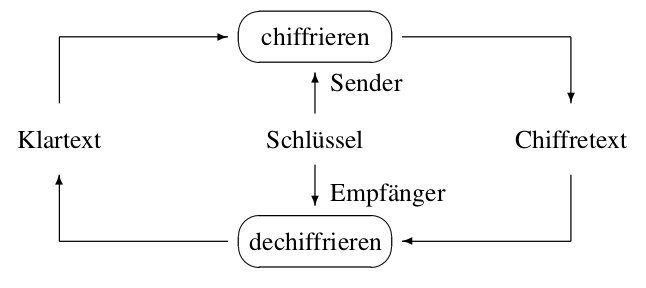
\includegraphics[scale=0.5]{figures/ver-und-entschluesseln.png}
			\quelle{(Wätjen, 2018, S.1)}
			\label{ver-und-entschluesselung}
			\caption{Symmetrische Ver- und Entschlüsselung}
		\end{minipage}
	\end{figure}	
	\subsection{RSA}
		Von asymmetrischer Verschlüsselung ist die Rede, wenn die Teilnehmer anstatt einen gemeinsamen Schlüssel zu haben, der im vor hinein ausgetauscht werden muss, jeder ein Schlüsselpaar (öffentlicher und privater Schlüssel) besitzt. Das \gls{rsa} Verfahren ist ein solches asymmetrisches Verschlüsselungsverfahren welches von den drei namens gebenden Mathematikern 1977 entwickelt wurde. Das \gls{rsa} Verfahren ist wohl das am häufigsten verwendete Public-Key-Kryptosystem.\\
		\textbf{Beispiel 1.} Die Gesprächspartner Alice und Bob, welche beide ein Schlüsselpaar besitzen, miteinander kommunizieren. Alice verschlüsselt einen Nachrichtentext mit dem öffentlichen Schlüssel von Bob und sendet die verschlüsselte Nachricht an Bob. Dieser kann seinerseits mit seinem privaten Schlüssel die Nachricht entschlüsseln.\footnote{Vgl. Dietmar Wätjen, 2018, S.73 f.}\\
	\subsection{Signaturen}
		Für die Sicherstellung der Authentizität können sogenannte Signaturen verwendet werden. Das oben kurz erläuterte Verfahren kann nicht nur zum Ver- und Entschlüsseln von Nachrichten benutzt werden, sondern auch zum signieren.\\
		Dabei wird statt des öffentlichen Schlüssels, der private Schlüssel benutzt um eine, in diesem Fall, Signatur zu erzeugen. Diese kann dann mit dem öffentlichen Schlüssel des zugehörigen privaten Schlüssels verifiziert werden.\\
		\textbf{Beispiel 2.} Bob möchte eine Nachricht an Alice schicken und sichergehen, dass diese auf dem Weg nicht verändert wurde. Er verwendet seinen privaten Schlüssel und wendet diesen auf eine Nachricht an um eine Signatur zu erzeugen. Beides übermittelt er an Alice. Mit dem öffentlichen Schlüssel von Bob kann die fehlerfreie Übertragung der Nachricht verifiziert werden.
		
\section{ActivityPub Standard}
	\iflanguage{english}{
		
	}{
		ActivityPub definiert zwei Protokollschichten, sowie Konzepte, Sammlungen und Interaktionen für dezentrale soziale Netzwerke. Eine Protokollschicht ist das Client-zu-Server Protokoll (Social API), um Clients den Zugriff auf einen Server zu ermöglichen sowie zum entgegennehmen von Anfragen. Die zweite Protokollschicht besteht aus dem förderierten Server-zu-Server Protkoll (Federation Protocol), welches den einzelnen Instanzen von dezentralen sozialen Netzwerken den Austausch von Inhalten untereinander gestattet. ActivityPub setzt auf bereits bestehende Empfehlungen des \gls{w3c} auf, welche teilweise auch von der \gls{swwg} entwickelt wurden wie zB. \gls{asc} und \gls{asv}.\\
		
		Auch andere Technologien wie \gls{JSON-LD} werden benutzt um die Erweiterbarkeit zu gewährleisten. Über neue Ontologien (Vokabulare) können weitere syntaktische Definitionen und semantische Beschreibungen zu den bestehenden hinzugefügt werden\cite{activityPub}. Diese Vokabulare können im Kontext des \gls{JSON-LD} Objektes, angegeben werden. Bei ActivityPub wird das \gls{AS2} Vokabular verwendet welches durch \gls{asv} erweitert wird.
	}
	\subsection{Bestandteile des Protokolls}
		Das Client-zu-Server sowie förderierte Server-zu-Server Protokoll können unabhängig voneinander implementiert werden. Ersteres besteht aus einem Client und Server Teil.\\
		
		In ActivityPub werden Benutzer als \glqq Aktoren\grqq(actors) dargestellt. Diese können nicht nur Personen, sondern auch Applikationen, Organisationen, Gruppen und Services sein\cite{activityStreamsCore}. Jedes Aktoren Objekt muss eine \glqq Inbox\grqq~und \glqq Outbox\grqq, welche geordnete Sammlungen sein müssen, sowie eine ID und ein Typ besitzen\cite{activityPub}. Die ID muss global einzigartig sein. Dies kann garantiert werden durch eine Domänen und Protokoll bezogene URI oder IRI wie zum Beispiel \glqq https://example.org/users/alice\grqq oder \glqq https://example.org/users/alice/áŷýà/2\grqq. %http://fusion.cs.uni-jena.de/fusion/blog/2016/11/18/iri-uri-url-urn-and-their-differences/
		Der Typ eines Aktor (z.B. "type": "Create") kann variieren zwischen den fünf oben genannten.
		
		\lstinputlisting{resources/mastodon-macu.json}
	
	\subsection{Authentifizierung und Datenintegrität}
		Für die Authentifizierung und zum sichern der Datenintegrität definiert der Standard keine Mechanismen. Es gibt allerdings \glqq Best Practices\grqq~für die Umsetzung dieser Anforderungen.\\
		
		Zum einen werden bei der Client-zu-Server Authentifizierung \glqq OAuth 2.0\grqq~Tokens benutzt, zum anderen auf der Server Seite \glqq HTTP\grqq~oder \glqq Linked Data Signatures\grqq zur Sicherstellung der Datenintegrität.\\
		\todo{OAuth 2.0}
		
		
		\todo{Datenintegrität}
		\glqq Die Datenintegrität umfasst Maßnahmen damit geschützte Daten während der Verarbeitung oder Übertragung nicht durch unautorisierte Personen entfernt oder verändert werden können. Sie stellt die Konsistenz, die Richtigkeit und Vertrauenswürdigkeit der Daten während deren gesamten Lebensdauer sicher und sorgt dafür, dass die relevanten Daten eines Datenstroms rekonstruierbar sind.\grqq\footnote{\cite{data-integrity}}
		
		\todo{HTTP Signaturen}
		Um sicherzustellen das HTTP Anfragen beim Transport nicht verändert wurden, können HTTP Signaturen verwendet werden. Bei diesen wird ein kryptografischer Algorithmus benutzt um \\
		
		\todo{Linked Data Signaturen}
		Wenn ein Objekt nicht nur vom Client zum Server gesendet, sondern auch zwischen Servern untereinander weitergeleitet werden soll wird zum Sicherstellen der Datenintegrität ein anderes Verfahren benötigt als HTTP Signaturen. Die \glqq Best Practices\grqq~empfehlen für solche Fälle \glqq Linked Data Signatures\grqq. Der größte Unterschied zwischen HTTP Signaturen und \glqq Linked Data Signatures\grqq~besteht darin, welche Daten zum Erstellen der Signatur verwendet werden. Bei HTTP Signaturen sind es die Kopfzeilen. Mit \glqq Linked Data Signatures\grqq~kann auch das Objekt selbst, also der Payload einer HTTP Anfrage, anstatt nur die Kopfzeilen, zum signieren verwendet werden.
	
	\subsection{Zugehörige Standards und Komponenten}
		ActivityPub benutzt die ActivityStreams Daten Syntax und das Vokabular. Zusätzlich kann ein weiteres Sicherheitsvokabular\footnote{Eine Ontologie die Sicherheitsaspekte definiert wie öffentliche Schlüssel, Signaturen u.v.m.} benutzt werden um Definitionen zum Bereitstellen eines öffentlichen Schlüssels, Signaturen sowie Verschlüsselten Inhalten u.v.m. zu haben. Am 22 April 2016 hat die \glqq W3C Community Group\grqq~ einen Entwurfsbericht herausgebracht. Durch diesen wird neue Syntax und Semantik definiert um Internet basierten Applikationen das Verschlüsseln, Entschlüsseln sowie digitale signieren und verifizieren von verlinkten Daten (Linked Data) zu ermöglichen. Es enthält auch Vokabeln für die Erstellung und Verwaltung einer dezentralen Public-Key-Infrastruktur über das Internet\cite{security-vocab-linked-data}. Ein Anwendungsfall ist das holen des öffentlichen Schlüssels eines Nutzers, über dessen Aktoren Objekt, um eine von Nutzer gesendete Nachricht zu verifizieren.
		
		\gls{JSON-LD} ist eine Erweiterung des JSON Formates um verlinkte Daten zu Repräsentieren. JSON an sich, ist ein Format welches im Web häufig Anwendung findet um Daten auszutauschen. Im Kern sind \gls{AS2} auch \gls{JSON-LD} Objekte. Der \gls{AS2} Kontext definiert verschiedene Klassen und Eigenschaften, von denen nicht alle benutzt werden. Typische Klassen sind \glqq Activity\grqq, \glqq Link\grqq~und \glqq OrderedCollection\grqq. Ein Beispiel \gls{AS2} Objekt sieht wie folgt aus: 	
		\lstinputlisting[caption={Beispiel \gls{AS2} Objekt}, label=listing::as2-object, language=Javascript]{resources/example-as2-object.json}

\section{Fediverse}
	Als erstes soll der Begriff \glqq förderiertes Netzwerk\grqq~von Förderation hergeleitet werden.\\
	
	Unter einer Förderation versteht man den Verbund von etwas. Deutschland ist z. B. ein förderierter Bundesstaat, welcher 16 Bundesländern verbindet. Ein Verbund von Netzwerken wird demnach als Netzwerkverbund, oder auch \glqq förderiertes Netzwerk\grqq,~bezeichnet.\\
	
	\glqq Fediverse\grqq~ist ein Kofferwort aus \glqq Federated\grqq~und \glqq Universe\grqq. Historisch gesehen beinhaltete der Begriff nur Microblogging Plattformen die das OStatus Protokoll unterstützen. Mehr zu OStatus \textbf{S. \ref{subsec:ostatus}}. Mittlerweile beinhaltet das Fediverse mehr als nur Microblogging Plattformen wie Mastodon\footnote{\url{https://mastodon.social/about}} sondern auch soziale Netzwerke (z. B. GNU Social\footnote{\url{https://gnu.io/social/}}), sowie \glqq Video hosting\grqq~(PeerTube\footnote{\url{https://joinpeertube.org/en/}}),\glqq Content publishing\grqq~Plattformen, wie Wordpress, und viele weitere.\cite{fediverse}\\
	
	Im \glqq Fediverse\grqq~dreht sich alles um freie (Open Source) Software anstelle von kommerziellen Produkten. Zudem kann ausgesucht werden welchem Administrator man die Kontrolle über seine Daten geben möchte, anstatt auf eine einzelne Instanz vertrauen zu müssen.\cite{fediverse}\\
	\todo{indirektes online Zitat!!!}
	
	Laut dem Fediverse Netzwerkreport 2018, welcher online zur Verfügung steht, hat sich die Gesamtanzahl der erreichbaren Instanzen von 2.756 auf 4.340 erhöht. Dies entspricht einem Wachstum von 58\%. Die Nutzeranzahl ist von 1.786.036 auf 2.474.601 gestiegen (39\%). Weitere Details sind im Netzwerk Report nachzulesen. Es ist hinzuzufügen das der Netzwerkreport unvollständig ist und Fehler beinhalten kann.\cite{fediverse-report}\\